در این پوشه به تمام مسیر‌های نرم‌افزار پرداخته شده است.

\begin{figure}[H]
	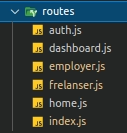
\includegraphics[width=.3\textwidth]{Folders-Files/routes.png}
	\centering
	\caption{ساختار پوشه مسیر}
	\label{fig:folder-routes}
\end{figure}

\subsection{فایل index}
در این فایل تمام آدرس‌های پوشه‌های مسیر برنامه قرار دارد.

\subsection{فایل home}
در این فایل به مسیر صفحه اصلی/اول/خانه پرداخته شده است.

\subsection{فایل auth}
در این فایل به مسیر ورود، ثبت‌نام و خروج پرداخته شده است.

\subsection{فایل dashboard}
در این فایل به مسیر داشبورد کاربر پرداخته شده است.

\subsection{فایل employer}
در این فایل به مسیر داشبورد کارفرما پرداخته شده است.

\subsection{فایل frelanser}
در این فایل به مسیر داشبورد فریلنسر پرداخته شده است.



checkdate
\\
 اعتبارسنجی تاریخ هجری شمسی
\\
توضیحات
\\
bool shcheckdate ( int \$year , int \$month , int \$day );
\lstdefinelanguage{JavaScript}{
	keywords={typeof, new, true, false, catch, function, return, null, catch, switch, var, if, in, while, do, else, case, break},
	keywordstyle=\color{blue}\bfseries,
	ndkeywords={class, export, boolean, throw, implements, import, this},
	ndkeywordstyle=\color{darkgray}\bfseries,
	identifierstyle=\color{black},
	sensitive=false,
	comment=[l]{//},
	morecomment=[s]{/*}{*/},
	commentstyle=\color{purple}\ttfamily,
	stringstyle=\color{red}\ttfamily,
	morestring=[b]',
	morestring=[b]"
}
\lstset{
	language=JavaScript,
	%backgroundcolor=\color{darkgray},
	extendedchars=true,
	basicstyle=\footnotesize\ttfamily,
	showstringspaces=false,
	showspaces=false,
	tabsize=2,
	breaklines=true,
	showtabs=false,
	captionpos=b
}
\begin{lstlisting}
			methodName: function(params){}
\end{lstlisting}

\mint{html}|<h2>Something <b>here</b></h2>|

بررسی اعتبار تاریخی که توسط آرگومان‌های تابع وارد می‌شود.در صورتی که پارامترها به درستی وارد شوند،یک تاریخ معتبر خواهد بود.
\\
\rule{\linewidth}{0.5mm}

پارامترها
\\
\begin{tabular}{|c|c|}
	\hline
	 پارامتر	& توضیحات \\
	\hline
	&  \\
	\hline
	&  \\
	\hline
\end{tabular}

برگردان
\\
در صورتی که تاریخ وارد شده معتبر باشد TRUE در غیر این صورت FALSE خواهد بود.

